\chapter{Preprocesamiento}

Esta clase tiene como objetivo comprender los pasos básicos de preprocesamiento de imágenes SAR. Para esto descargaremos imágenes de la web y las procesaremos a los distintos niveles de corrección geométrica y radiométrica.

\section{Descarga de imágenes}

Para descargar imágenes SAR utilizaremos el catálogo del \href{https://vertex.daac.asf.alaska.edu/}{Alaska Satellite Facility}. Dirijase a la página y en la sección de \emph{Geographic Region} seleccione un area que incluya a la ciudad de Ushuaia (Figura \ref{fig:region}).

\begin{figure}[h!]
    \centering
    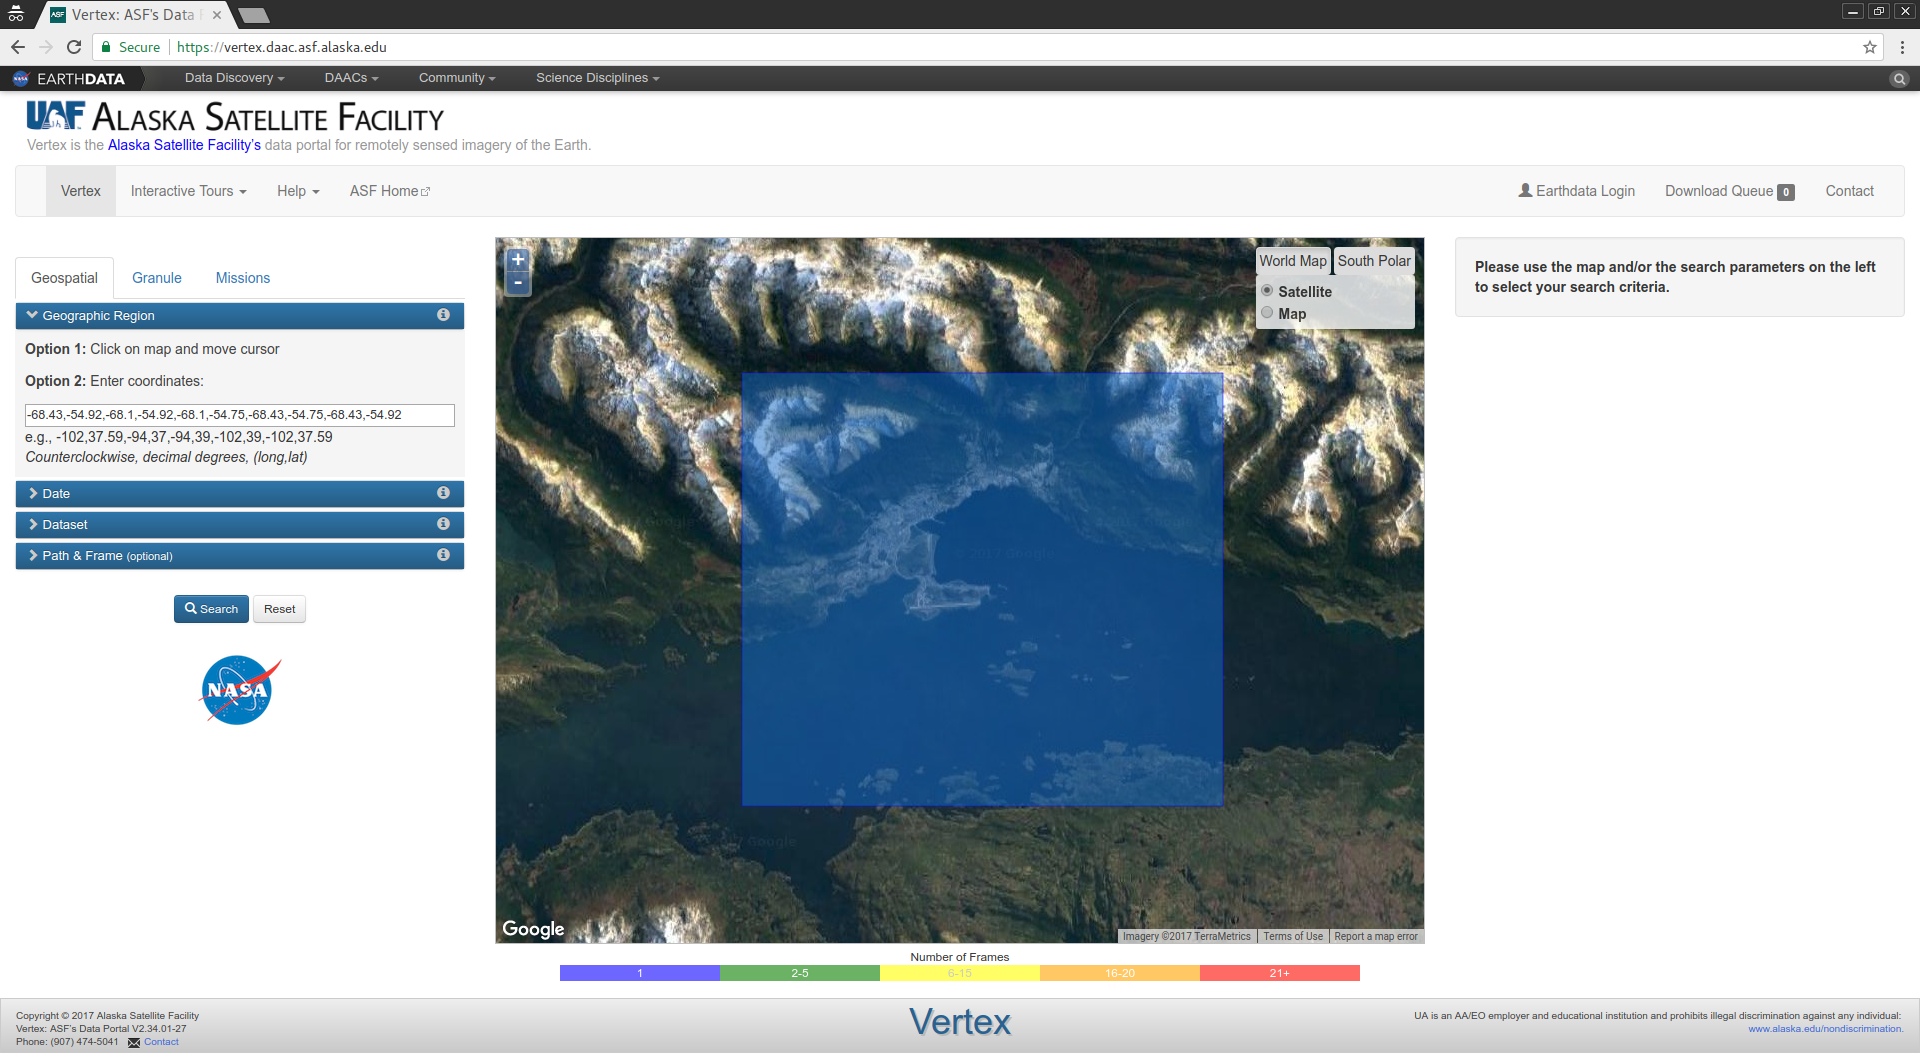
\includegraphics[width=0.5\textwidth]{fig:region.png}
    \caption{}
    \label{fig:region}
\end{figure}

Seleccione luego en \emph{Dataset} el set de datos de \emph{ALOS PALSAR} (Figura \ref{fig:dataset}) y haga click en search.

\begin{figure}[h!]
    \centering
    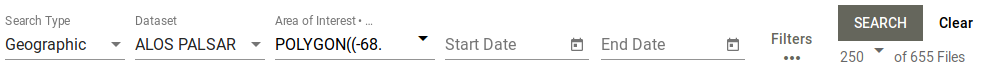
\includegraphics[width=0.5\textwidth]{fig:dataset.png}
    \caption{}
    \label{fit:dataset}
\end{figure}

Aparecera a la derecha de la pantalla una lista de producto. Seleccione de ellos el de nombre \emph{ALOS PALSAR PLR} del 20 de abril del 2040 pertenenciente al frame 6070 y el path 119 (Figura \ref{fig:dataset}).

Descarge el producto \emph{Level 1.1 Complex (661.42 MB)} (Figura \ref{fig:descarga}). En caso de que el sistema así se lo pida, registrese.

\begin{figure}[h!]
    \centering
    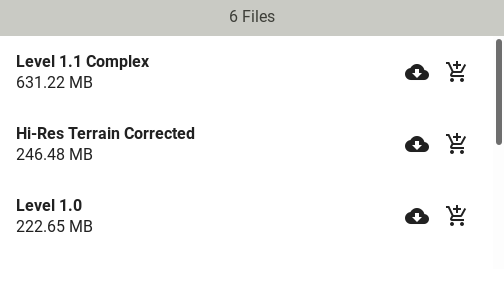
\includegraphics[width=0.5\textwidth]{fig:descarga.png}
    \caption{}
    \label{fig:descarga}
\end{figure}

El producto descargado corresponde a una imagen \emph{Single look complex} en \emph{slant range}.

\section{Calibración}

Abra la imagen \path{ALPSRP278916070-L1.1.zip} que descargo del Alaska Satellite Facility. Despliegue la banda \path{intensity_HH} y observe que se encuentra comprimida horizontalmente.

Para calibrar la imagen, dirijase al menu \emph{Radar, Radiometric, Calibrate} (Figura \ref{fig:calibrar}).

 \begin{figure}[h!]
     \centering
     \includegraphics{fig:calibrar.png}
     \caption{}
     \label{fig:calibrar}
 \end{figure}

 Obtendrá una imagen calibrada con los coeficientes de backscatter \path{sigma_0_HH_dB}. En este caso verá 4 bandas correspondientes a 4 formas de interacción entre el blanco y la radiación. Será cada una tema de nuestra próxima clase.

 \section{Filtrado}

 Para disminuir el ruido speckle en la imagen hay dos procesos que podemos realizar.

 \subsection{Multilooking}

 El proceso de multilooking genera una nueva imagen a partir de los pixeles en una ventana. Para realizarlo seleccione la herramienta \emph{Radar, Multilooking}.

 Seleccione en source la imagen \path{ALOS-P1_1__A-ORBIT__ALPSRP278916070_Cal} que generó en el paso anterior. Es posible seleccionar en este caso el numero de looks y sobre que bandas se realizarán. Pongalo igual a 1. En caso de no seleccionar ninguna el proceso se aplicará sobre todas las bandas (Figura \ref{fig:multilook}).

\begin{figure}[h!]
    \centering
    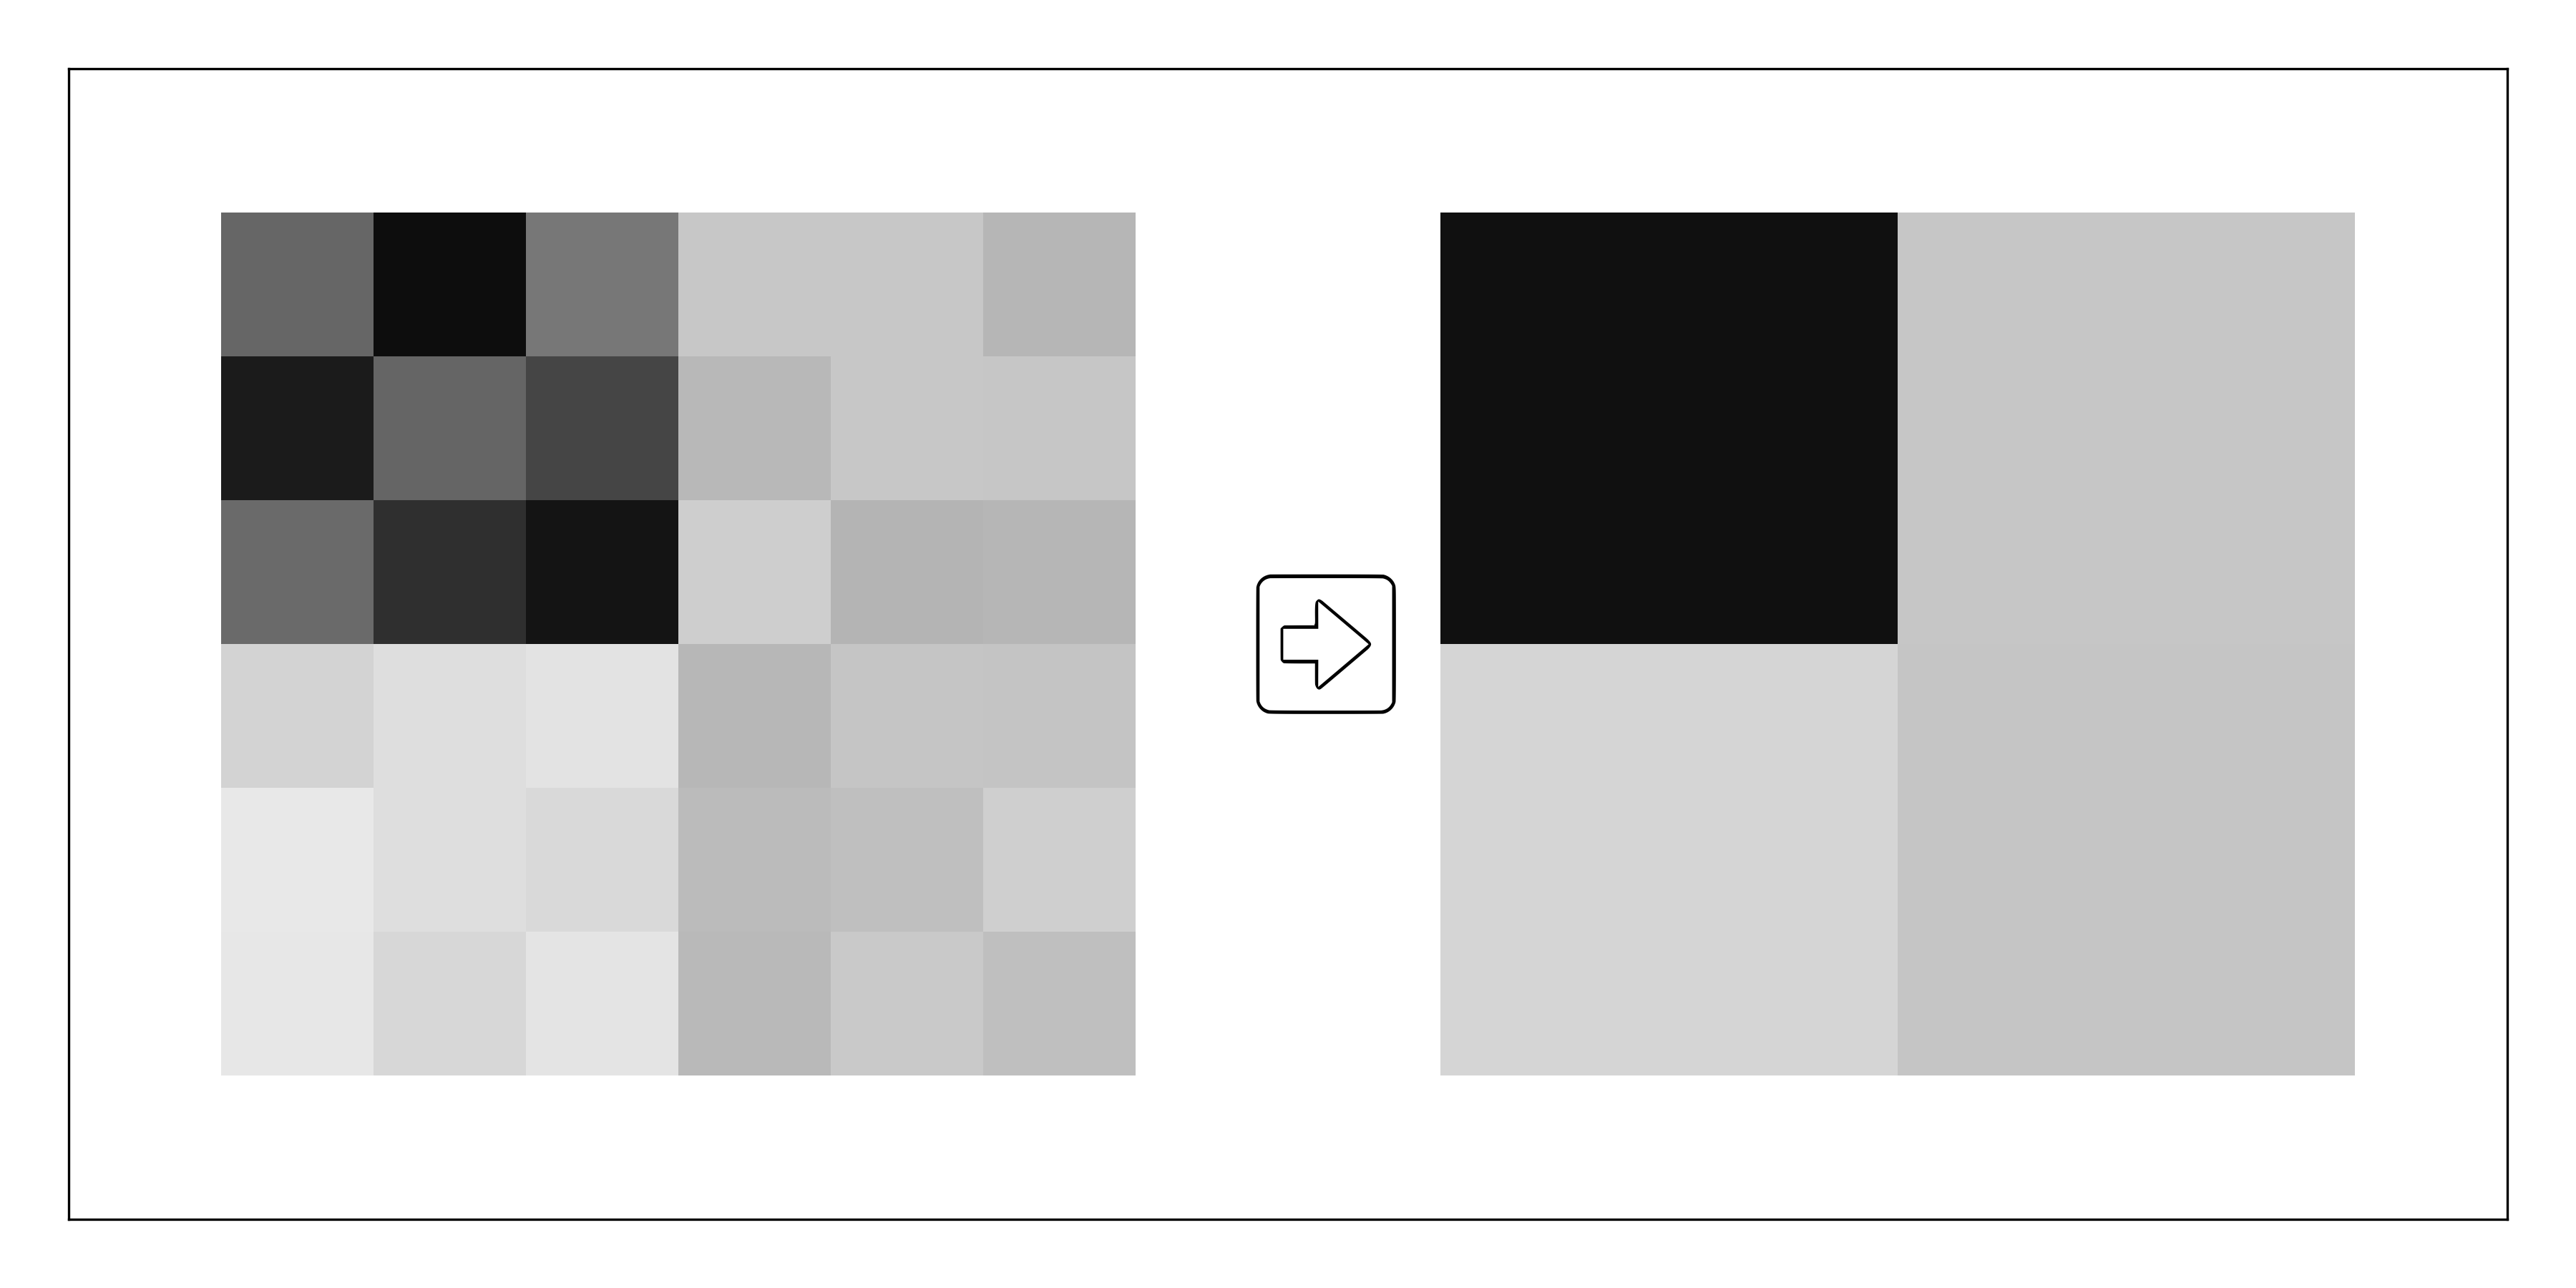
\includegraphics{fig:multilook.png}
    \caption{}
    \label{fig:multilook}
\end{figure}

\begin{que}
Observe la banda \path{sigma_0_HH} de la imagen multilookeada.
\end{que}


\subsection{Speckle filter}

Existen otros filtros que ayudan a disminuir el ruido de la imagen. Uno de los más comunes es el filtro \emph{Lee Sigma}. Para aplicarlo a la imagen multilookeada vaya al menu \emph{Radar, Speckle Filter, Single Product Speckle Filter}.

Seleccione en source la imagen \path{ALOS-P1_1__A-ORBIT__ALPSRP278916070_Cal_ML} que generó al aplicar el multilook. En processing parameter elija el filtro de \emph{Lee Sigma} con un numero de looks igual a 1 y una ventana de 7x7 (Figura \ref{fig:lee})

\begin{figure}[h!]
    \centering
    \includegraphics{fig:lee.png}
    \caption{}
    \label{fig:lee}
\end{figure}

\begin{que}
    Observe y compare la banda \path{sigma_0_HH} de la imagen filtrada con la imagen multilookeada.
\end{que}

\section{Proyección}

Finalmente es es común proyectar la imagen del \emph{slant range} al \emph{ground range}. Esta imagen podrá después ser abierta en cualquier softwarae de GIS sin problemas. Para hacerlo existen dos opciones: proyectar la imagen sobre el elipsoide o sobre un modelo de elevación digital.

Para el caso de las imágenes ALOS PALSAR 1, es necesario previamente aplicar un procesor antes de proyectarlas en el terreno. Este proceso se llama \emph{deskewing}. Para hacerlo vaya al menu \emph{Radar, Geometric, ALOS deskewing} y ejecute el proceso sobre la imagen \path{ALOS-P1_1__A-ORBIT__ALPSRP278916070_Cal_ML_Spk}.

\subsection{Elipsoide - GEC}

Al proyectar la imagen sobre el elipsoide podremos hacerlo sobre cualquier lugar del planeta. Perderemos al hacerlo la información sobre el relieve local que es de importancia al momento de utilizar imagenes SAR.

Para hacerlo, vaya al menú \emph{Radar, Geometric, Ellipsoid Correction, Average Height Range Doppler}. Seleccione la imagen \path{ALOS-P1_1__A-ORBIT__ALPSRP278916070_Cal_ML_Spk_DSk} y deje los parametros por defecto (Figura \ref{fig:elipsoide}).

\begin{figure}[h!]
    \centering
    \includegraphics{fig:elipsoide.png}
    \caption{}
    \label{fig:elipsoide}
\end{figure}

\begin{que}
    ¿Que sucede con la imagen luego de la proyección?
\end{que}

\subsection{Elipsoide - GTC}

Al proyectar la imagen sobre un modelo de elevación digital estaremos teniendo en cuenta la elevación del lugar al pasar al terreno desde la proyección del rango. Esto mejorara algunos aspectos de la imagen como el forshortening y el foreshadowinf.

Para hacerlo, vaya al menú \emph{Radar, Geometric, Terrain Correction, Range Doppler Terrain Correction}. Seleccione la imagen \path{ALOS-P1_1__A-ORBIT__ALPSRP278916070_Cal_ML_Spk_DSk} y en \emph{processing parameters} destilde la opción \emph{Mask out areas without elevation} (Figuraa \ref{fig:gtc}).

\begin{figure}[h!]
    \centering
    \includegraphics{fig:gtc.png}
    \caption{}
    \label{fig:gtc}
\end{figure}

\begin{que}
    ¿Que sucede con la imagen luego de la proyección?
\end{que}

\section{dB}

Puede convertir la imagen a dB en cualquier momento haciendo click derecho sobre la banda y seleccionando la opción \emph{Linear to/from dB}.

Convierta a dB la banda \path{sigma_0_HH} y explore visualmente la imagen obtenida. Conviene siempre explorar las imagenes en dB pues es una medida más natural para nuestro ojo. Sin embargo, al momento de realizar procesamiento, conviene utilizar la imagen sin hacerlo.

\section{Actividades}

\begin{que}
    Compare visualmente las imágenes TC y EC obtenidas por los métodos anteriores. ¿Que sucede con las montañas? ¿Hacia donde parecen estar inclinadas?
\end{que}

\begin{que}
    ¿Porque las montañas parecen mas brillantes de un lado que del otro?
\end{que}

\begin{que}
    Obtenga los valores de dB para las coberturas de agua, urbano y bosque.
\end{que}

\begin{que}
    Dentro del agúa encontrará un punto muy brillante cerca de la ciudad de Ushuahia. ¿A que se debe este punto? ¿Que aplicación le encuentra a las imagenes SAR para detectar objetos sobre el agua?
\end{que}
